\documentclass[12pt,a4paper]{article}

% ─── Page Layout ───────────────────────────────────────────────────────────────
\usepackage[a4paper, margin=0.8in, headheight=14pt]{geometry}

% ─── Fonts (XeLaTeX) ───────────────────────────────────────────────────────────
\usepackage{fontspec}
\usepackage{unicode-math}
\setmainfont{TeX Gyre Pagella}
\setmonofont[Scale=0.88]{TeX Gyre Cursor}
\setmathfont{Latin Modern Math}

% ─── Packages ──────────────────────────────────────────────────────────────────
\usepackage{xcolor}
\usepackage{colortbl}
\usepackage{titlesec}
\usepackage{enumitem}
\usepackage{tabularx}
\usepackage{booktabs}
\usepackage{array}
\usepackage{amsmath}
\usepackage{tikz}
\usetikzlibrary{shapes.geometric, arrows.meta, positioning, calc, fit, decorations.pathreplacing, decorations.pathmorphing}
\usepackage{tcolorbox}
\tcbuselibrary{skins, breakable}
\usepackage{hyperref}
\usepackage{fancyhdr}
\usepackage{graphicx}
\usepackage{microtype}
\hyphenpenalty=10000
\exhyphenpenalty=10000
\sloppy
\usepackage{caption}
\usepackage{setspace}
\usepackage{multirow}
\usepackage{tocloft}

% ─── Q&A helper ────────────────────────────────────────────────────────────────
\newcommand{\Q}[1]{\textbf{#1}\par\noindent\ignorespaces}

% ─── Colour Palette ────────────────────────────────────────────────────────────
\definecolor{myred}{RGB}{196,30,58}
\definecolor{mydark}{RGB}{30,30,50}
\definecolor{mygreen}{RGB}{14,120,80}
\definecolor{myteal}{RGB}{0,130,140}
\definecolor{myamber}{RGB}{180,100,0}
\definecolor{mypurple}{RGB}{100,30,160}
\definecolor{mygray}{RGB}{246,247,249}
\definecolor{mgframe}{RGB}{180,185,200}
\definecolor{watermark}{RGB}{145,150,170}
\definecolor{hdrred}{RGB}{250,232,235}
\definecolor{hdrgreen}{RGB}{220,244,233}
\definecolor{hdrteal}{RGB}{220,242,244}
\definecolor{hdramber}{RGB}{253,242,215}
\definecolor{hdrpurple}{RGB}{238,228,255}
\definecolor{hdrgray}{RGB}{238,240,245}
\definecolor{rowalt}{RGB}{250,251,253}

% ─── Section Formatting ────────────────────────────────────────────────────────
\titleformat{\section}
  {\large\bfseries\color{myred}}{\thesection.}{0.5em}{}
  [\vspace{1pt}{\color{myred}\rule{\linewidth}{0.8pt}}]
\titleformat{\subsection}
  {\normalsize\bfseries\color{myteal}}{\thesubsection}{0.5em}{}
\titlespacing*{\section}{0pt}{18pt}{7pt}
\titlespacing*{\subsection}{0pt}{11pt}{4pt}

% ─── Paragraph ─────────────────────────────────────────────────────────────────
\setlength{\parindent}{0pt}
\setlength{\parskip}{4pt}

% ─── TOC Styling ───────────────────────────────────────────────────────────────
\renewcommand{\cfttoctitlefont}{\large\bfseries\color{myred}}
\renewcommand{\cftaftertoctitle}{\par\noindent{\color{myred}\rule{\linewidth}{0.8pt}}}
\setlength{\cftbeforetoctitleskip}{0pt}
\setlength{\cftaftertoctitleskip}{6pt}
\renewcommand{\cftsecfont}{\normalsize\bfseries\color{mydark}}
\renewcommand{\cftsecpagefont}{\normalsize\bfseries\color{mydark}}
\renewcommand{\cftsecleader}{\cftdotfill{\cftdotsep}}
\setlength{\cftbeforesecskip}{7pt}
\renewcommand{\cftsubsecfont}{\small\color{mydark}}
\renewcommand{\cftsubsecpagefont}{\small\color{mydark}}
\setlength{\cftbeforesubsecskip}{3pt}
\setlength{\cftsubsecindent}{1.4em}

% ─── Table helpers ─────────────────────────────────────────────────────────────
\renewcommand{\arraystretch}{1.45}
\setlength{\tabcolsep}{6pt}
\arrayrulecolor{mydark}
\newcolumntype{B}[1]{>{\small\bfseries\raggedright\arraybackslash}m{#1}}
\newcolumntype{C}[1]{>{\centering\arraybackslash}m{#1}}
\newcolumntype{Y}{>{\small\raggedright\arraybackslash}X}
\renewcommand{\tabularxcolumn}[1]{m{#1}}

% ─── Header / Footer ───────────────────────────────────────────────────────────
\pagestyle{fancy}
\fancyhf{}
\fancyhead[L]{\small\color{myred}\textbf{OE-EC704A}\;\color{mydark}--- Web Technology}
\fancyhead[R]{\small\color{myteal}\textbf{Module 7 Notes}}
\fancyfoot[C]{\small\color{mydark}\thepage}
\fancyfoot[R]{\small\color{watermark}\textit{\copyright\ Biraj}}
\renewcommand{\headrulewidth}{0.5pt}
\renewcommand{\footrulewidth}{0.3pt}

% ─── Hyperref ──────────────────────────────────────────────────────────────────
\hypersetup{
  colorlinks=true, linkcolor=myteal, urlcolor=myteal,
  pdfauthor={Biraj Sarkar},
  pdftitle={OE-EC704A --- Module 7 Notes}
}

% ─── tcolorbox styles ──────────────────────────────────────────────────────────
\tcbset{
  tikzbox/.style={
    colback=mygray, colframe=mgframe, boxrule=0.6pt, arc=4pt,
    left=8pt, right=8pt, top=6pt, bottom=6pt,
    colbacktitle=mgframe, coltitle=mydark,
    fonttitle=\small\bfseries
  },
  defbox/.style={
    colback=hdrgreen, colframe=mygreen, boxrule=0.8pt, arc=4pt,
    left=9pt, right=9pt, top=6pt, bottom=6pt,
    colbacktitle=mygreen, coltitle=white,
    fonttitle=\small\bfseries
  },
  formulabox/.style={
    colback=hdrteal, colframe=myteal, boxrule=0.8pt, arc=4pt,
    left=9pt, right=9pt, top=7pt, bottom=7pt,
    colbacktitle=myteal, coltitle=white,
    fonttitle=\small\bfseries
  },
  examplebox/.style={
    colback=hdramber, colframe=myamber, boxrule=0.8pt, arc=4pt,
    left=9pt, right=9pt, top=6pt, bottom=6pt,
    colbacktitle=myamber, coltitle=white,
    fonttitle=\small\bfseries
  },
  masonbox/.style={
    colback=hdrpurple, colframe=mypurple, boxrule=0.8pt, arc=4pt,
    left=9pt, right=9pt, top=6pt, bottom=6pt,
    colbacktitle=mypurple, coltitle=white,
    fonttitle=\small\bfseries
  },
  exambox/.style={
    colback=hdrpurple, colframe=mypurple, boxrule=1pt, arc=5pt,
    left=10pt, right=10pt, top=8pt, bottom=8pt,
    colbacktitle=mypurple, coltitle=white,
    fonttitle=\bfseries,
    breakable, title after break={\textbf{Frequently Asked / Viva Questions (contd.)}}}
}
\tcbset{breakable}

% ─── TikZ styles ───────────────────────────────────────────────────────────────
\tikzset{
  block/.style={rectangle, draw=myteal, fill=hdrteal,
    text width=2.5cm, align=center, minimum height=1.0cm,
    font=\small, rounded corners=3pt, line width=0.7pt},
  redblock/.style={rectangle, draw=myred, fill=hdrred,
    text width=2.5cm, align=center, minimum height=1.0cm,
    font=\small, rounded corners=3pt, line width=0.7pt},
  netnode/.style={rectangle, draw=myteal, fill=hdrteal,
    text width=1.8cm, align=center, minimum height=0.8cm,
    font=\small, rounded corners=3pt, line width=0.7pt},
  sumjunc/.style={circle, draw=myamber, fill=hdramber,
    minimum size=0.6cm, font=\small, line width=0.8pt},
  snode/.style={circle, draw=mypurple, fill=hdrpurple,
    minimum size=0.55cm, font=\footnotesize, line width=0.7pt},
  arrow/.style={-Stealth, thick, color=mydark},
  redarrow/.style={-Stealth, thick, color=myred},
  line/.style={thick, color=mydark}
}

% ═══════════════════════════════════════════════════════════════════════════════
\begin{document}
% ═══════════════════════════════════════════════════════════════════════════════

\begin{center}
  {\LARGE\bfseries\color{myred} OE-EC704A --- Web Technology}\\[5pt]
  {\normalsize\color{mydark} Semester VII \quad$\bullet$\quad 3L:0T:0P \quad$\bullet$\quad 3 Credits}\\[3pt]
  {\normalsize\color{myteal}\textbf{Module 7 Exam Notes: Java I/O Streams}}\\[3pt]
  {\small\color{mydark} CGEC \;$|$\; B.Tech ECE (2023--27) \;$|$\; \textit{Biraj Sarkar}}
\end{center}
\noindent{\color{myred}\rule{\linewidth}{1.5pt}}
\vspace{2pt}

\hypersetup{linkcolor=mydark}
\tableofcontents
\hypersetup{linkcolor=myteal}
\newpage

% ===============================================================================
\section{Java I/O Stream Basics}
% ===============================================================================

An Input/Output (I/O) Stream represents an abstraction of a data source (e.g., keyboard, file) or destination (e.g., console, network socket).

\begin{tcolorbox}[defbox, title={\textbf{Stream Concept}}]
A \textbf{Stream} is a continuous sequence of data bytes. Input streams are used to read data from a source, and Output streams are used to write data to a target.
\end{tcolorbox}

\subsection{Byte Stream vs. Character Stream}
Java's I/O library operates on two primary categories of streams:
\begin{itemize}[leftmargin=*, itemsep=3.5pt]
  \item \textbf{Byte Streams:} Process data as raw 8-bit bytes. They are suitable for binary data (images, sound, zip files).
  \item \textbf{Character Streams:} Process data as 16-bit Unicode characters. They handle translation of text encoding models automatically.
\end{itemize}

\begin{tcolorbox}[tikzbox, title={Java Stream Hierarchy}]
\centering
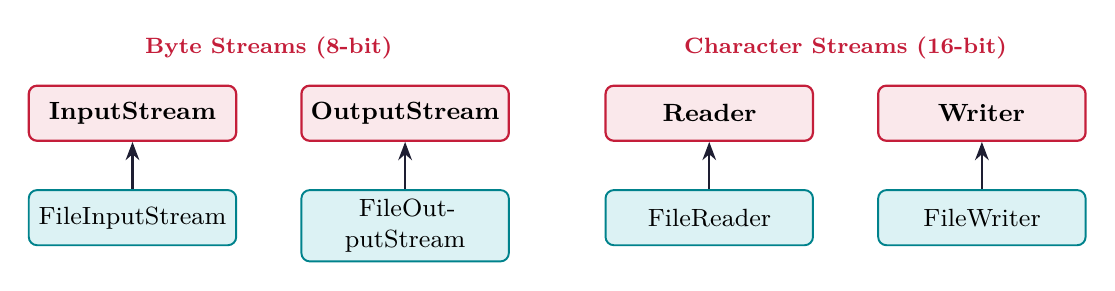
\begin{tikzpicture}[node distance=0.8cm and 1.2cm,
  base/.style={rectangle, draw=myred, fill=hdrred, text width=2.4cm,
    align=center, minimum height=0.7cm, font=\small\bfseries, rounded corners=3pt, line width=0.8pt},
  sub/.style={rectangle, draw=myteal, fill=hdrteal, text width=2.4cm,
    align=center, minimum height=0.7cm, font=\small, rounded corners=3pt, line width=0.7pt}]

  % Byte Streams
  \node[base] (is) {InputStream};
  \node[sub, below=0.6cm of is] (fis) {FileInputStream};
  \draw[arrow] (fis) -- (is);
  
  \node[base, right=0.8cm of is] (os) {OutputStream};
  \node[sub, below=0.6cm of os] (fos) {FileOutputStream};
  \draw[arrow] (fos) -- (os);

  % Character Streams
  \node[base, right=1.2cm of os] (rd) {Reader};
  \node[sub, below=0.6cm of rd] (fr) {FileReader};
  \draw[arrow] (fr) -- (rd);
  
  \node[base, right=0.8cm of rd] (wr) {Writer};
  \node[sub, below=0.6cm of wr] (fw) {FileWriter};
  \draw[arrow] (fw) -- (wr);

  % Labels
  \node[above=0.2cm of $(is.north)!0.5!(os.north)$, font=\footnotesize\bfseries, color=myred] {Byte Streams (8-bit)};
  \node[above=0.2cm of $(rd.north)!0.5!(wr.north)$, font=\footnotesize\bfseries, color=myred] {Character Streams (16-bit)};
\end{tikzpicture}
\end{tcolorbox}

% ===============================================================================
\section{Console I/O Operations}
% ===============================================================================

Java represents console streams using three static variables declared in the \texttt{System} class:
\begin{itemize}[leftmargin=*, itemsep=3pt]
  \item \textbf{\texttt{System.in}:} Standard Input Stream (type \texttt{InputStream}), mapped to keyboard input.
  \item \textbf{\texttt{System.out}:} Standard Output Stream (type \texttt{PrintStream}), mapped to console output.
  \item \textbf{\texttt{System.err}:} Standard Error Stream (type \texttt{PrintStream}), mapped to console error output.
\end{itemize}

\subsection{Reading Console via BufferedReader}
Because \texttt{System.in} is a byte stream, we wrap it in a character stream (\texttt{InputStreamReader}) and pass it to a \texttt{BufferedReader} to enable line-by-line reading:
\begin{verbatim}
BufferedReader br = new BufferedReader(new InputStreamReader(System.in));
System.out.print("Enter your name: ");
String name = br.readLine();
\end{verbatim}

\subsection{Reading Console via Scanner}
The \texttt{java.util.Scanner} class parses primitives and strings using regular expressions:
\begin{verbatim}
Scanner sc = new Scanner(System.in);
System.out.print("Enter an integer: ");
int value = sc.nextInt();
\end{verbatim}

% ===============================================================================
\section{File I/O Operations}
% ===============================================================================

\subsection{FileInputStream and FileOutputStream}
Used to read and write raw bytes from/to a file on disk:
\begin{verbatim}
// Copying a binary file byte-by-byte
try (FileInputStream fis = new FileInputStream("input.jpg");
     FileOutputStream fos = new FileOutputStream("output.jpg")) {
    int byteData;
    while ((byteData = fis.read()) != -1) {
        fos.write(byteData);
    }
} catch (IOException e) {
    e.printStackTrace();
}
\end{verbatim}

\subsection{FileReader and FileWriter}
Used to read and write character text data from/to files on disk:
\begin{verbatim}
try (FileReader fr = new FileReader("file.txt");
     FileWriter fw = new FileWriter("copy.txt")) {
    int charData;
    while ((charData = fr.read()) != -1) {
        fw.write(charData);
    }
} catch (IOException e) {
    e.printStackTrace();
}
\end{verbatim}

\subsection{Buffered Stream Wrapper Pattern}
Disk I/O requests are expensive. To improve performance, we wrap base stream classes inside buffered wrapper classes:
\begin{itemize}[leftmargin=*, itemsep=3.5pt]
  \item \textbf{\texttt{BufferedReader}:} Wraps around a \texttt{Reader} (e.g., \texttt{FileReader}) to buffer characters, providing a highly efficient \texttt{readLine()} method.
  \item \textbf{\texttt{BufferedWriter}:} Wraps around a \texttt{Writer} to buffer written characters, writing to disk only when the buffer is full or when \texttt{flush()} is invoked.
\end{itemize}

\newpage
% ===============================================================================
\begin{center}
  {\large\bfseries\color{myred} Quick Revision --- Module 7}\\[3pt]
  {\small\color{mydark} Java I/O Streams $|$ OE-EC704A}
\end{center}
\noindent{\color{myred}\rule{\linewidth}{1.2pt}}
\vspace{4pt}

\begin{tcolorbox}[formulabox, title={\textbf{Java I/O Stream Syntax}}]
{\renewcommand{\arraystretch}{1.3}%
\begin{tabularx}{\linewidth}{l Y}
\textbf{Construct} & \textbf{Syntax and Example Usage} \\
\hline
Console BufferedReader & \texttt{BufferedReader br = new BufferedReader(new InputStreamReader(System.in));} \\
Console Scanner & \texttt{Scanner sc = new Scanner(System.in); int val = sc.nextInt();} \\
File Reader (Text) & \texttt{FileReader fr = new FileReader("input.txt"); int c = fr.read();} \\
File Writer (Text) & \texttt{FileWriter fw = new FileWriter("output.txt"); fw.write("Hello");} \\
File Byte Input & \texttt{FileInputStream fis = new FileInputStream("in.dat"); fis.read();} \\
Buffered Writer Wrapper & \texttt{BufferedWriter bw = new BufferedWriter(new FileWriter("out.txt"));} \\
\end{tabularx}}
\end{tcolorbox}

\begin{tcolorbox}[defbox, title={\textbf{One-Line Definitions}}]
\begin{itemize}[leftmargin=*, itemsep=2pt]
  \item \textbf{Stream:} A logical abstraction of a continuous sequence of data bytes.
  \item \textbf{Byte Stream:} Stream processing raw 8-bit binary data units.
  \item \textbf{Character Stream:} Stream processing 16-bit Unicode character data units.
  \item \textbf{InputStreamReader:} A bridge class converting byte streams into character streams.
  \item \textbf{BufferedReader:} A character stream wrapper that caches characters in memory to reduce disk calls.
  \item \textbf{Scanner:} A text scanner utility class parsing primitives using token delimiters.
  \item \textbf{System.in:} Static instance of InputStream mapped to the client keyboard.
  \item \textbf{System.out:} Static instance of PrintStream mapped to the standard console output.
\end{itemize}
\tcbset{after={\color{black}}}
\end{tcolorbox}

\begin{tcolorbox}[exambox, title={\textbf{Frequently Asked / Viva Questions}}]
\begin{enumerate}[leftmargin=*, label=\textbf{Q\arabic*.}, itemsep=5pt]
  \item \Q{What is the difference between Byte Streams and Character Streams?}
        Byte streams read/write data as 8-bit bytes (base classes: \texttt{InputStream}, \texttt{OutputStream}), ideal for binary files. Character streams read/write data as 16-bit Unicode characters (base classes: \texttt{Reader}, \texttt{Writer}), ideal for text files.
        
  \item \Q{Why do we wrap a \texttt{FileReader} inside a \texttt{BufferedReader}?}
        Reading directly from disk is slow. Wrapping in a \texttt{BufferedReader} caches character chunks in memory, reducing physical disk reads, and exposes the convenient \texttt{readLine()} method.
        
  \item \Q{What is the purpose of the \texttt{InputStreamReader} class?}
        It acts as a bridge, converting a byte stream (like \texttt{System.in}) into a character stream, translating bytes into characters using the default system charset.
        
  \item \Q{What is the difference between \texttt{PrintStream} and \texttt{PrintWriter}?}
        \texttt{PrintStream} is a byte stream class handling 8-bit output (like \texttt{System.out}). \texttt{PrintWriter} is a character stream class handling 16-bit Unicode character output.
        
  \item \Q{What does the method \texttt{flush()} do in output streams?}
        It forces the output stream to write any cached buffered bytes/characters immediately to the destination device (like the disk file), emptying the local memory buffer.
        
  \item \Q{What is the default buffer size of a \texttt{BufferedReader}?}
        The default buffer size is 8192 characters (8 KB), which is large enough to handle most typical text file read sizes efficiently.
        
  \item \Q{How does the \texttt{Scanner} class handle delimiters?}
        By default, the \texttt{Scanner} class uses whitespace (spaces, tabs, newlines) as the token delimiter. This can be customized using the \texttt{useDelimiter()} method.
        
  \item \Q{What is the difference between \texttt{read()} method of \texttt{InputStream} and \texttt{Reader}?}
        \texttt{InputStream.read()} reads a single byte and returns it as an integer ($0$ to $255$). \texttt{Reader.read()} reads a single Unicode character and returns it as an integer ($0$ to $65535$). Both return $-1$ when reaching EOF.
        
  \item \Q{What checked exception is commonly thrown during file operations?}
        \texttt{java.io.IOException} and its subclass \texttt{java.io.FileNotFoundException}. They must be explicitly caught or declared using a \texttt{throws} clause.
        
  \item \Q{What are the standard console stream fields inside the \texttt{System} class?}
        \texttt{System.in} (standard input - \texttt{InputStream}), \texttt{System.out} (standard output - \texttt{PrintStream}), and \texttt{System.err} (standard error - \texttt{PrintStream}).
\end{enumerate}
\end{tcolorbox}

\begin{tcolorbox}[tikzbox, title={Comparison: Reader/Writer vs. InputStream/OutputStream}]
\centering
{\renewcommand{\arraystretch}{1.45}%
\begin{tabularx}{\linewidth}{|B{3.2cm}|Y|Y|}
\hline
\textbf{Metric} & \textbf{Reader / Writer Hierarchy} & \textbf{InputStream / OutputStream Hierarchy} \\
\hline
\textbf{Data Unit} & 16-bit Unicode character unit. & 8-bit raw byte unit. \\
\hline
\textbf{Primary Target} & Text documents and strings. & Images, sound, ZIP, raw binary data. \\
\hline
\textbf{Root Packages} & Lives inside \texttt{java.io} & Lives inside \texttt{java.io} \\
\hline
\textbf{Default EOF value} & Returns $-1$ at stream end. & Returns $-1$ at stream end. \\
\hline
\end{tabularx}}
\tcbset{after={\color{black}}}
\end{tcolorbox}

\end{document}
